\section{Consuntivo di periodo - Preventivo a finire}
In questa sezione viene presentato il bilancio tra il preventivo e il consuntivo. Tale bilancio può essere:
\begin{itemize}
	\item \textbf{Positivo}: il preventivo ha superato il consuntivo;
	\item \textbf{Negativo}: il consuntivo ha superato il preventivo;
	\item \textbf{In pari}: il consuntivo coincide con il preventivo.
\end{itemize}

\subsection{Analisi dei Requisiti}
Di seguito verrà presentato il consuntivo per l'attività di \textit{\AdR}.
\\\\
La tabella sottostante riporta le ore preventivate e, tra parentesi, la differenza di tali ore con quelle effettivamente impiegate per ciascun componente del gruppo \gruppo.

\begin{table}[H]
	\begin{center}
		\begin{tabular}{|c|c|c|c|c|c|c|c|}
			\hline
			\textbf{Nominativo} & \multicolumn{6}{c|}{\textbf{Ore per ruolo}} & \textbf{Ore totali} \\
			& \textbf{Re} & \textbf{Am} & \textbf{An} & \textbf{Pj} & \textbf{Pr} & \textbf{Ve} & \\
			\hline	
			\FB		&			&	4 (+1)	&	23		&		&		&		&	27 (+1)	\\
			\hline
			\AF		&			&	6 		&	21		&	 	&		&		& 	27		\\
			\hline
			\GN		&	20		&			&	9 (+2)	&		&		&		&	29		\\
			\hline
			\GR		&	20 (+1)	&	 		&	8 		&		&	 	& 		&	28		\\
			\hline
			\SM 	&			&	3		&	5		&		&		& 	20	&	28		\\
			\hline
			\MP		& 			&			&	7		&		&		&	20	&	27 (+1)	\\
			\hline
			\MV 	&			&	4		&	5		&		&		&	20	& 	29		\\
			\hline
		\end{tabular}
	\end{center}
	\caption{Differenza preventivo-consuntivo per componente, \AdR}
\end{table}



La tabella sottostante, invece, riporta le ore preventivate e  tra parentesi la differenza di ore tra preventivo e consuntivo, divise per ruolo.

\begin{table}[H]
	\begin{center}
		\begin{tabular}{|l|c|c|}
			\hline
			\textbf{Ruolo}	& \textbf{Ore} & \textbf{Costo} \\
			\hline
			\textit{Responsabile}		&	40 (+1)	&	1200 (+30)	\\
			\hline
			\textit{Amministratore}		&	17 (+1)	&	340 (+20)	\\
			\hline
			\textit{Analista}			&	78 (+2)	&	1950 (+50)	\\
			\hline
			\textit{Verificatore}		&	60 (+1)	&	900 (+15)	\\
			\hline
			\textbf{Totale preventivo}	&	195		&	4390 		\\
			\hline
			\textbf{Totale consuntivo}	&	200		&   4505		\\
			\hline
			\textbf{Differenza} 		&	-5		&	-115		\\
			\hline
		\end{tabular}
	\end{center}
	\caption{Differenza preventivo-consuntivo per ruolo, \AdR}
\end{table}
 
\subsubsection{Conclusioni}

Come mostrato dalla tabella, risulta che il gruppo ha utilizzato complessivamente cinque ore un più rispetto alla pianificazione nel periodo di \textit{Analisi dei Requisiti}, con un bilancio in passivo pari a 115€. Tale passivo non andrà influenzare il costo totale del progetto in quanto le ore impiegate in questo periodo non vengono poste a carico del proponente.

\subsection{Analisi dei Requisiti in Dettaglio}
Di seguito verrà presentato il consuntivo per l'attività di \textit{\AD}.
\\\\
La tabella sottostante riporta le ore preventivate e, tra parentesi, la differenza di tali ore con quelle effettivamente impiegate per ciascun componente del gruppo \gruppo.

\begin{table}[H]
	\begin{center}
		\begin{tabular}{|c|c|c|c|c|c|c|c|}
			\hline
			\textbf{Nominativo} & \multicolumn{6}{c|}{\textbf{Ore per ruolo}} & \textbf{Ore totali} \\
			& \textbf{Re} & \textbf{Am} & \textbf{An} & \textbf{Pj} & \textbf{Pr} & \textbf{Ve} & \\
			\hline
			\FB			&			&		&	3 (-2)	&		&		&			&	3 (-2)	\\
			\hline
			\AF			&			&		&	3 (-1)	&	 	&		&			& 	3 (-1)		\\
			\hline
			\GN			&	1 		&		&			&		&		&			&	1		\\
			\hline
			\GR			&	2 (-2)	&	 	&	 		&		&	 	& 			&	2 (-2)	\\
			\hline
			\SM 		&			&	1	&			&		&		& 	1		&	2		\\
			\hline
			\MP			& 			&		&			&		&		&	3 (-2)	&	3 (-2)	\\
			\hline
			\MV 		&			&		&			&		&		&	1		& 	1		\\
			\hline
		\end{tabular}
	\end{center}
	\caption{Differenza preventivo-consuntivo per componente, \AD}
\end{table}

La tabella sottostante, invece, riporta le ore preventivate e  tra parentesi la differenza di ore tra preventivo e consuntivo, divise per ruolo.

\begin{table}[H]
	\begin{center}
		\begin{tabular}{|l|c|c|}
			\hline
			\textbf{Ruolo}	& \textbf{Ore} & \textbf{Costo} \\
			\hline
			\textit{Responsabile}		&	3 (-2)	&	90 (-60) 	\\
			\hline
			\textit{Amministratore}		&	1		&	20 			\\
			\hline
			\textit{Analista}			&	6 (-3)	&	150 (-75) 	\\
			\hline
			\textit{Verificatore}		&	5 (-2)	&	75 (-30)	\\
			\hline
			\textbf{Totale preventivo}	&	15		& 	335			\\
			\hline
			\textbf{Totale consuntivo}	&	8		&  	170			\\
			\hline
			\textbf{Differenza} 		&	7		&	165			\\
			\hline
		\end{tabular}
	\end{center}
	\caption{Differenza preventivo-consuntivo per ruolo, \AD}
\end{table}

\subsubsection{Conclusioni}
Come mostrato dalla tabella, risulta che il gruppo ha utilizzato complessivamente 7 ore in meno rispetto la pianificazione dell'attività di \textit{\AD}, con un bilancio in attivo pari a 165€, che sommato al bilancio dell'attività di \textit{\AR} risulta un attivo di 50€.

\newpage
\subsection{Progettazione Architetturale}

Di seguito verrà presentato il consuntivo per l'attività di \textit{\PA}.
\\\\
La tabella sottostante riporta le ore preventivate e, tra parentesi, la differenza di tali ore con quelle effettivamente impiegate per ciascun componente del gruppo \gruppo.

\begin{table}[H]
	\begin{center}
		\begin{tabular}{|c|c|c|c|c|c|c|c|}
			\hline
			\textbf{Nominativo} & \multicolumn{6}{c|}{\textbf{Ore per ruolo}} & \textbf{Ore totali} \\
			& \textbf{Re} & \textbf{Am} & \textbf{An} & \textbf{Pj} & \textbf{Pr} & \textbf{Ve} & \\
			\hline
			\FB			&		&		&		&	10(-3)	&		&	23	&	33(-3)	\\
			\hline
			\AF			&		&		&		&	9(+2) 	&		&	23	& 	32(+2)	\\
			\hline
			\GN			&		&		&		&	8	&		&	24	&	32	\\
			\hline
			\GR			&		&	4	&  		&	28	&	 	& 		&	32	\\
			\hline
			\SM 		&	3(-1)	&		&		&	29	&		& 		&	32(-1)	\\
			\hline
			\MP 		& 		&	4	&		&	28	&		&		&	32	\\
			\hline
			\MV 		&	3	&		&		&	29	&		&		& 	32	\\
			\hline
		\end{tabular}
	\end{center}
	\caption{Differenza preventivo-consuntivo per componente, Progettazione Architetturale}
\end{table}

\begin{figure}[H]
	\centering
	\includegraphics[scale=0.4]{immagini/Grafi/ProgettazioneArchitetturale_oreComponente.png}
	\caption{Differenza preventivo-consuntivo per componente, Progettazione Architetturale}
\end{figure}
\FloatBarrier

\newpage
La tabella sottostante, invece, riporta le ore preventivate e  tra parentesi la differenza di ore tra preventivo e consuntivo, divise per ruolo.

\begin{table}[H]
	\begin{center}
		\begin{tabular}{|l|c|c|}
			\hline
			\textbf{Ruolo}	& \textbf{Ore} & \textbf{Costo} \\
			\hline
			\textit{Responsabile}		&	6 (-1)	&	180 (-30) 	\\
			\hline
			\textit{Amministratore}		&	8		&	160			\\
			\hline
			\textit{Progettista}		&	141 (-1)&	3102 (-22) 	\\
			\hline
			\textit{Verificatore}		&	70 		&	1050 		\\
			\hline
			\textbf{Totale preventivo}	&	225		& 	4492		\\
			\hline
			\textbf{Totale consuntivo}	&	222		&  	4440		\\
			\hline
			\textbf{Differenza} 		&	2		&	52			\\
			\hline
		\end{tabular}
	\end{center}
	\caption{Differenza preventivo-consuntivo per ruolo, \PA}
\end{table}

\begin{figure}[H]
	\centering
	\includegraphics[scale=0.4]{immagini/Grafi/ProgettazioneArchitetturale_oreRuolo.png}
	\caption{Differenza preventivo-consuntivo per ruolo, Progettazione Architetturale}
\end{figure}
\FloatBarrier

\subsubsection{Conclusioni}

Come mostrato dalla tabella, risulta che il gruppo ha utilizzato complessivamente 2 ore in meno rispetto la pianificazione dell'attività di \textit{\PA}, con un bilancio in attivo pari a 52€.

\subsubsection{Preventivo a finire}
Da quanto riportato precedentemente si evince la possibilità di impiegare la parte di budget risparmiato nelle fasi successive. \\
I \textbf{52€} verranno utilizzati per aumentare le ore di progettazione nella \textbf{\PD} permettendo di migliorare la qualità dei prodotti in ingresso alla \textit{Revisione di Progettazione} in vista dalla progettazione massima.

\newpage
\subsection{Progettazione di Dettaglio}
Di seguito verrà presentato il consuntivo per l'attività di \textit{\PD}.
\\\\
La tabella sottostante riporta le ore preventivate e, tra parentesi, la differenza di tali ore con quelle effettivamente impiegate per ciascun componente del gruppo \gruppo.

\begin{table}[H]
	\begin{center}
		\begin{tabular}{|c|c|c|c|c|c|c|c|}
			\hline
			\textbf{Nominativo} & \multicolumn{6}{c|}{\textbf{Ore per ruolo}} & \textbf{Ore totali} \\
			& \textbf{Re} & \textbf{Am} & \textbf{An} & \textbf{Pj} & \textbf{Pr} & \textbf{Ve} & \\
			\hline
			\FB			&	3		&			&		&	17 (+3)	&		&		&	20 (+3)		\\
			\hline
			\AF			&	4 (-2)	&			&		&	16 		&		&		& 	20 (-2)		\\
			\hline
			\GN			&			&	2		&		&	18		&		&		&	20			\\
			\hline
			\GR			&			&	 		&		&	6		&	 	& 	14	&	20			\\
			\hline
			\SM 		&			&	3 (+1)	&		&	17		&		& 		&	20 (+1)		\\
			\hline
			\MP 		& 			&			&		&	6		&		&	14	&	20			\\
			\hline
			\MV 		&			&			&		&	6		&		&	14	& 	20			\\
			\hline
		\end{tabular}
	\end{center}
	\caption{Differenza preventivo-consuntivo per componente, Progettazione di Dettaglio}
\end{table}

\begin{figure}[H]
	\centering
	\includegraphics[scale=0.4]{immagini/Grafi/ProgettazioneDettaglio_oreComponente.png}
	\caption{Differenza preventivo-consuntivo per componente, Progettazione di Dettaglio}
\end{figure}
\FloatBarrier

\newpage
La tabella sottostante, invece, riporta le ore preventivate e  tra parentesi la differenza di ore tra preventivo e consuntivo, divise per ruolo.

\begin{table}[H]
	\begin{center}
		\begin{tabular}{|l|c|c|}
			\hline
			\textbf{Ruolo}	& \textbf{Ore} & \textbf{Costo} \\
			\hline
			\textit{Responsabile}		&	7 (-2)	&	210 (-60) 		\\
			\hline
			\textit{Amministratore}		&	5 (+1)	&	100	(+20)		\\
			\hline
			\textit{Progettista}		&	86 (+3)	&	1892 (+66) 		\\
			\hline
			\textit{Verificatore}		&	42 		&	630 			\\
			\hline
			\textbf{Totale preventivo}	&	140		& 	2832			\\
			\hline
			\textbf{Totale consuntivo}	&	142		&  	2858			\\
			\hline
			\textbf{Differenza} 		&	-2		&	-26				\\
			\hline
		\end{tabular}
	\end{center}
	\caption{Differenza preventivo-consuntivo per ruolo, \PD}
\end{table}

\begin{figure}[H]
	\centering
	\includegraphics[scale=0.4]{immagini/Grafi/ProgettazioneDettaglio_oreRuolo.png}
	\caption{Differenza preventivo-consuntivo per ruolo, Progettazione in Dettaglio}
\end{figure}
\FloatBarrier

\subsubsection{Conclusioni}
Come mostrato dalla tabella, risulta che il gruppo ha utilizzato complessivamente 2 ore in più rispetto la pianificazione dell'attività di \textit{\PD}, con un bilancio in passivo pari a 26€, che sommato al bilancio all'attività di \textit{\PA} risulta un attivo di 26€.

\subsubsection{Preventivo a finire}
Da quanto riportato precedentemente si evince la possibilità di impiegare la parte di budget risparmiato nelle fasi successive. \\
I \textbf{26€} verranno utilizzati per aumentare le ore di programmazione nella \textbf{Codifica} permettendo di migliorare la qualità dei prodotti in ingresso alla \textit{Revisione di Qualifica}.

\newpage
\subsection{Codifica}
Di seguito verrà presentato il consuntivo per l'attività di \textit{Codifica}.
\\\\
La tabella sottostante riporta le ore preventivate e, tra parentesi, la differenza di tali ore con quelle effettivamente impiegate per ciascun componente del gruppo \gruppo.


\begin{table}[H]
	\begin{center}
		\begin{tabular}{|c|c|c|c|c|c|c|c|}
			\hline
			\textbf{Nominativo} & \multicolumn{6}{c|}{\textbf{Ore per ruolo}} & \textbf{Ore totali} \\
			& \textbf{Re} & \textbf{Am} & \textbf{An} & \textbf{Pj} & \textbf{Pr} & \textbf{Ve} & \\
			\hline
			\FB			&			&			&			&		&	35			&			&	35		\\
			\hline
			\AF			&			&			&			&	5	&	31			&			& 	36		\\
			\hline		
			\GN			&			&	4		&			&		&	7			&	25 (-3)	&	36 (-3)	\\
			\hline
			\GR			&	5		&	 		&			&	5	&	25 (+2) 	& 			&	35 (+2)	\\
			\hline
			\SM 		&			&			&			&	5	&	5			& 	25		&	35		\\
			\hline
			\MP 		& 	6 (-1)	&			&			&	5	&	24			&			&	35 (-1)	\\
			\hline
			\MV 		&			&			&			&	5	&	6			&	25 (+1)	& 	36 (+1)\\
			\hline
		\end{tabular}
	\end{center}
	\caption{Differenza preventivo-consuntivo per componente, Codifica}
\end{table}


\begin{figure}[H]
	\centering
	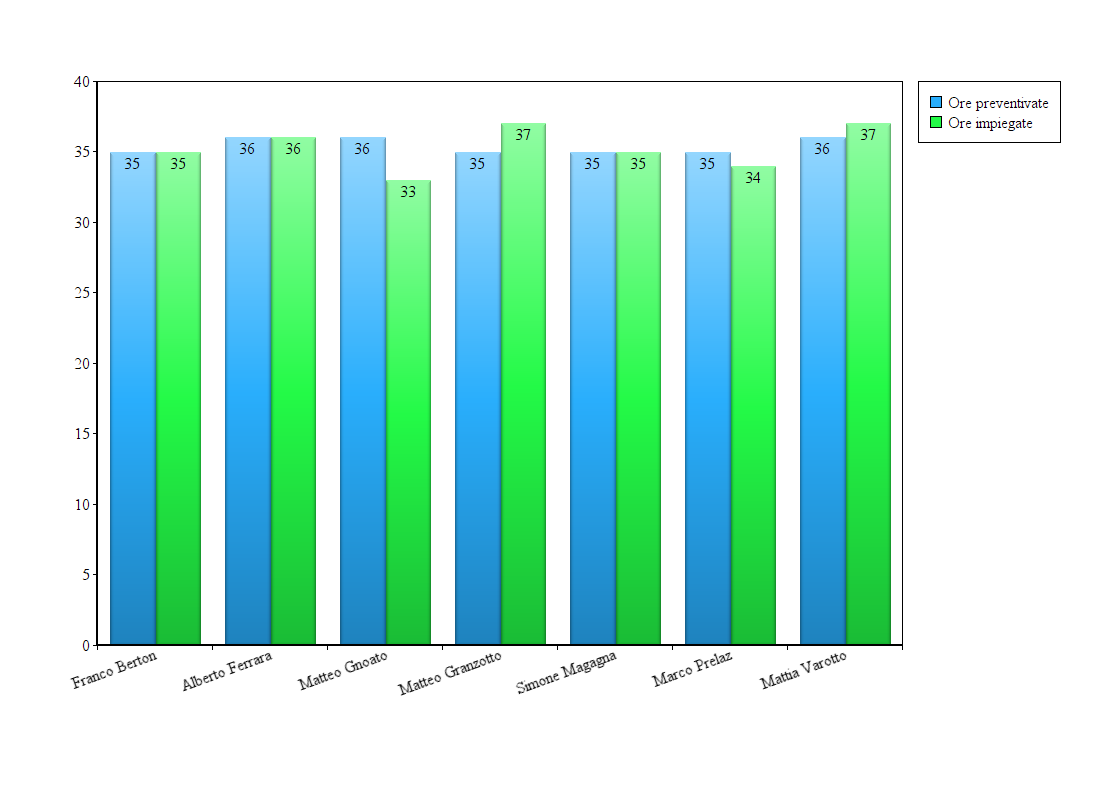
\includegraphics[scale=0.4]{immagini/Grafi/Codifica_oreComponente.png}
	\caption{Differenza preventivo-consuntivo per componente, Codifica}
\end{figure}
\FloatBarrier

\newpage
La tabella sottostante, invece, riporta le ore preventivate e  tra parentesi la differenza di ore tra preventivo e consuntivo, divise per ruolo.

\begin{table}[H]
	\begin{center}
		\begin{tabular}{|l|c|c|}
			\hline
			\textbf{Ruolo}	& \textbf{Ore} & \textbf{Costo} 		\\
			\hline
			\textit{Responsabile}		&	11 (-1)	&	330 (-30)	\\
			\hline
			\textit{Amministratore}		&	4		&	80			\\
			\hline
			\textit{Progettista}		&	25		&	550			\\
			\hline
			\textit{Programmatore}		&	133	(+2)&	1995 (+30)	\\
			\hline
			\textit{Verificatore}		&	75	(-2)&	1125 (-30)	\\
			\hline
			\textbf{Totale preventivo}	&	248		& 	4080		\\
			\hline
			\textbf{Totale consuntivo}	&	247		&  	4050		\\
			\hline
			\textbf{Differenza} 		&	1		&	30			\\
			\hline
		\end{tabular}
	\end{center}
	\caption{Differenza preventivo-consuntivo per ruolo, Codifica}
\end{table}

\begin{figure}[H]
	\centering
	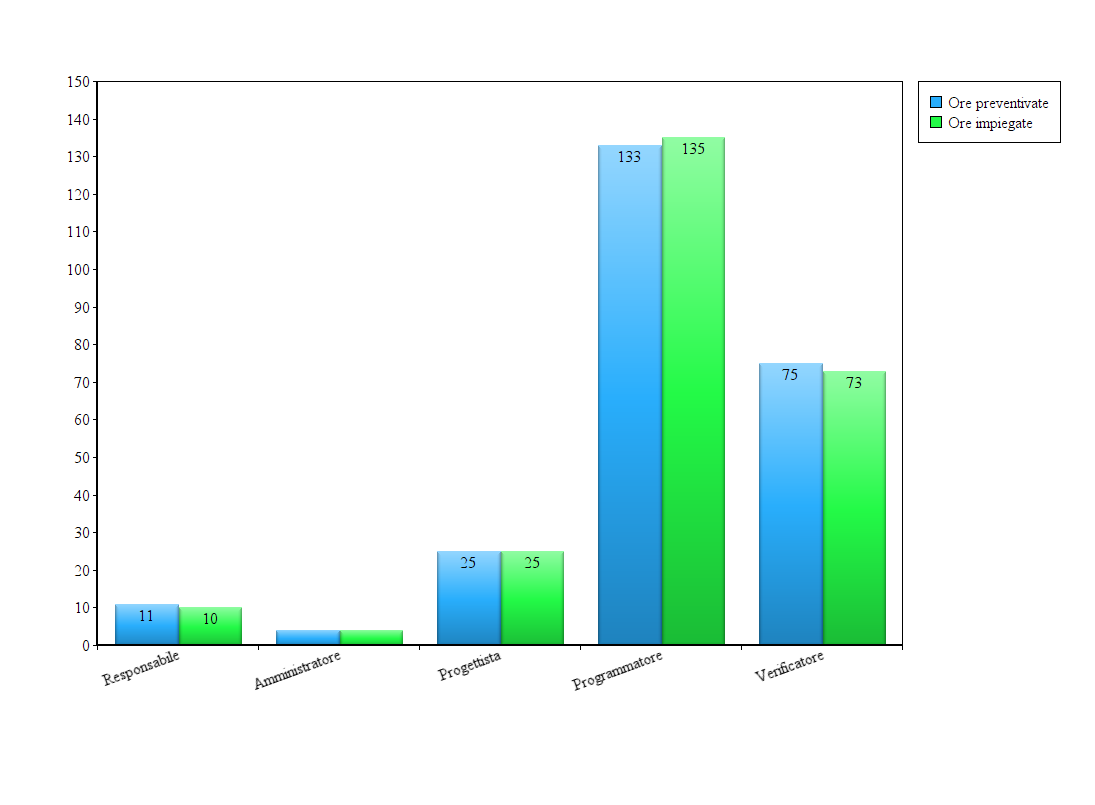
\includegraphics[scale=0.4]{immagini/Grafi/Codifica_oreRuolo.png}
	\caption{Differenza preventivo-consuntivo per ruolo, Codifica}
\end{figure}
\FloatBarrier

\subsubsection{Conclusioni}
Come mostrato dalla tabella, risulta che il gruppo ha utilizzato complessivamente 1 ora in meno rispetto la pianificazione dell'attività di \textit{Codifica}, con un bilancio in attivo pari a 30€, che sommato al bilancio all'attività di \textit{\PD} risulta un attivo di 56€.

\subsubsection{Preventivo a finire}
Da quanto riportato precedentemente si evince la possibilità di impiegare la parte di budget risparmiato nelle fasi successive. \\
I \textbf{56€} verranno utilizzati per aumentare le ore di verifica nella \textbf{Validazione} permettendo di migliorare la qualità dei prodotti in ingresso alla \textit{Revisione di Accettazione}.

\newpage
\subsection{Validazione}
Di seguito verrà presentato il consuntivo per l'attività di \textit{Validazione}.
\\\\
La tabella sottostante riporta le ore preventivate e, tra parentesi, la differenza di tali ore con quelle effettivamente impiegate per ciascun componente del gruppo \gruppo.

\begin{table}[H]
	\begin{center}
		\begin{tabular}{|c|c|c|c|c|c|c|c|}
			\hline
			\textbf{Nominativo} & \multicolumn{6}{c|}{\textbf{Ore per ruolo}} & \textbf{Ore totali} \\
			& \textbf{Re} & \textbf{Am} & \textbf{An} & \textbf{Pj} & \textbf{Pr} & \textbf{Ve} & \\
			\hline
			\FB			&			&			&			&	6		&			&	11			&	17				\\
			\hline
			\AF			&			&			&			&	6		&			&	11			& 	17				\\
			\hline		
			\GN			&			&			&			&	8		&			&	9 (+3)		&	17 (+3)			\\
			\hline
			\GR			&			&	 		&			&			&			& 	18 (-2)		&	18 (-2)			\\
			\hline
			\SM 		&	9		&			&			&			&			& 	9			&	18				\\
			\hline
			\MP 		& 			&			&			&			&			&	18 (+1)		&	17 (+1)			\\
			\hline
			\MV 		&			&			&			&			&			&	17	(-1)	& 	17 (-1)			\\
			\hline
		\end{tabular}
	\end{center}
	\caption{Differenza preventivo-consuntivo per componente, Validazione}
\end{table}

\begin{figure}[H]
	\centering
	\includegraphics[scale=0.4]{immagini/Grafi/Validazione_oreComponente.png}
	\caption{Differenza preventivo-consuntivo per componente, Validazione}
\end{figure}
\FloatBarrier

\newpage
La tabella sottostante, invece, riporta le ore preventivate e  tra parentesi la differenza di ore tra preventivo e consuntivo, divise per ruolo.

\begin{table}[H]
	\begin{center}
		\begin{tabular}{|l|c|c|}
			\hline
			\textbf{Ruolo}	& \textbf{Ore} & \textbf{Costo} 		\\
			\hline
			\textit{Responsabile}		&	9		&	270			\\
			\hline
			\textit{Progettista}		&	20		&	440			\\
			\hline
			\textit{Verificatore}		&	93 (+1)	&	1395 (+15)	\\
			\hline
			\textbf{Totale preventivo}	&	122		& 	2105		\\
			\hline
			\textbf{Totale consuntivo}	&	123		&  	2120		\\
			\hline
			\textbf{Differenza} 		&	-1		&	-15			\\
			\hline
		\end{tabular}
	\end{center}
	\caption{Differenza preventivo-consuntivo per ruolo, Validazione}
\end{table}

\begin{figure}[H]
	\centering
	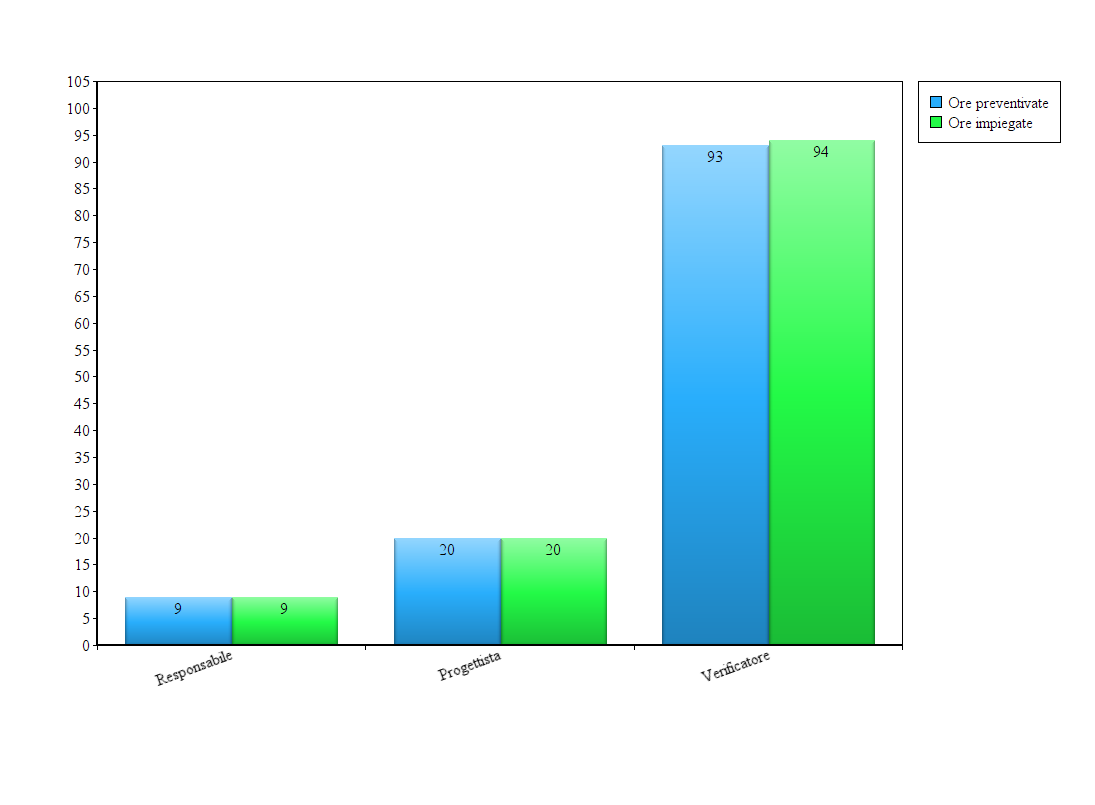
\includegraphics[scale=0.4]{immagini/Grafi/Validazione_oreRuolo.png}
	\caption{Differenza preventivo-consuntivo per ruolo, Validazione}
\end{figure}
\FloatBarrier

\subsubsection{Conclusioni}
Come mostrato dalla tabella, risulta che il gruppo ha utilizzato complessivamente 1 ora in più rispetto la pianificazione dell'attività di \textit{\VV}, con un bilancio in passivo pari a 15€, che sommato al bilancio all'attività di \textit{Codifica} risulta un attivo di 37€.

\newpage
\subsection{Totale}

Si riporta di seguito il consuntivo dell'intero sviluppo del progetto. \\
\\
La tabella sottostante riporta le ore preventivate e, tra parentesi, la differenza di tali ore con quelle effettivamente impiegate per ciascun componente del gruppo \gruppo.

\begin{table}[H]
	\begin{center}
		\begin{tabular}{|c|c|c|c|c|c|c|c|}
			\hline
			\textbf{Nominativo} & \multicolumn{6}{c|}{\textbf{Ore per ruolo}} & \textbf{Ore totali} \\
			& \textbf{Re} & \textbf{Am} & \textbf{An} & \textbf{Pj} & \textbf{Pr} & \textbf{Ve} & \\
			\hline
			\FB			&	3 (0)		&	0 (0)		&	0 (0)	 	&	33 (0)		&	35 (0)		&	34 (0)		&	105 (0)				\\
			\hline
			\AF			&	2 (-2)		&	0 (0)		&	0 (0)		&	37 (+2)		&	31 (0)		&	34 (0)		& 	105 (0)				\\
			\hline		
			\GN			&	0 (0)		&	6 (0)		&	0 (0)		&	34 (0)		&	7 (0)		&	58	(0)		&	105 (0)				\\
			\hline
			\GR			&	5 (0)		&	4 (0) 		&	0 (0)		&	39 (0)		&	27 (+2)		& 	30	(-2)	&	105 (0)				\\
			\hline
			\SM 		&	11 (-1)		&	4 (+1)		&	0 (0)		&	51 (0)		&	5 (0)		& 	34 (0)		&	105 (0)				\\
			\hline
			\MP 		& 	5 (-1)		&	4 (0)		&	0 (0)		&	39 (0)		&	24 (0)		&	33	(+1)	&	105 (0)				\\
			\hline
			\MV 		&	3 (0)		&	0 (0)		&	0 (0)		&	40 (0)		&	6 (0)		&	56	(0)		& 	105 (0)				\\
			\hline
		\end{tabular}
	\end{center}
	\caption{Differenza preventivo-consuntivo per componente, Totale}
\end{table}

\begin{figure}[H]
	\centering
	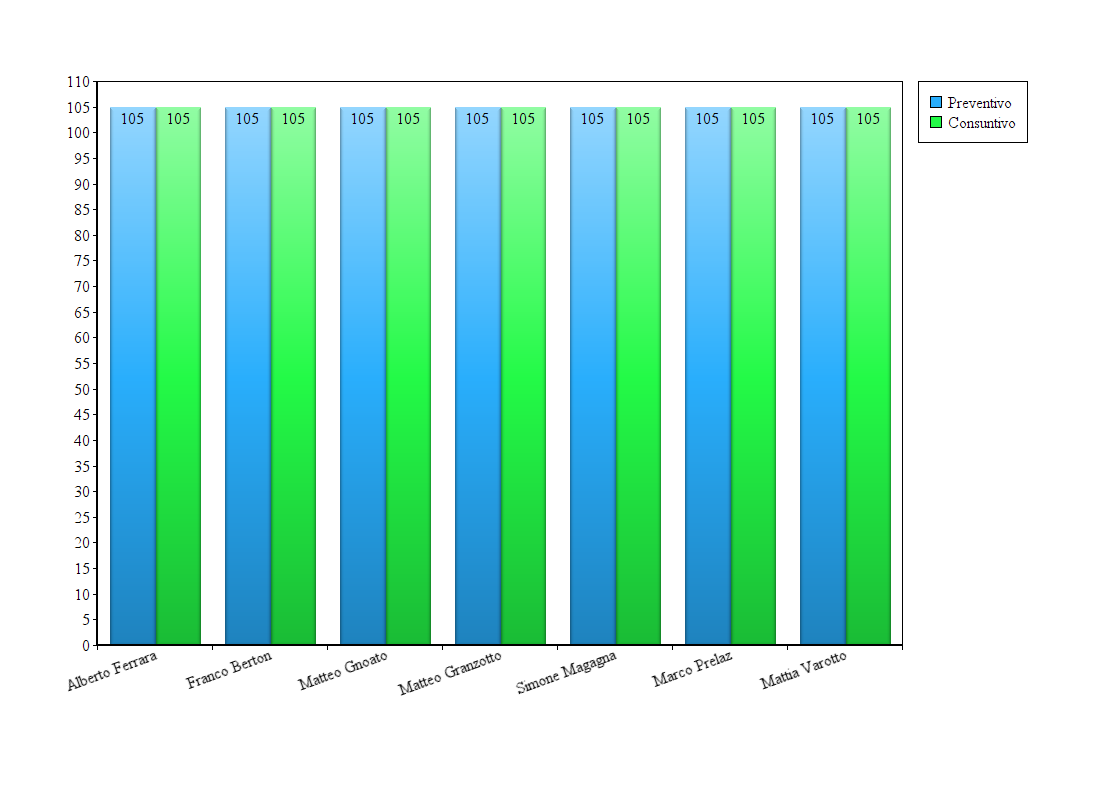
\includegraphics[scale=0.4]{immagini/Grafi/Totale_oreComponente.png}
	\caption{Differenza preventivo-consuntivo per componente, Totale}
\end{figure}
\FloatBarrier

\newpage
La tabella sottostante, invece, riporta le ore preventivate e  tra parentesi la differenza di ore tra preventivo e consuntivo, divise per ruolo.

\begin{table}[H]
	\begin{center}
		\begin{tabular}{|l|c|c|}
			\hline
			\textbf{Ruolo}	& \textbf{Ore} & \textbf{Costo} 					\\
			\hline
			\textit{Responsabile}		&	33 (-4)			&	990	(-120)		\\
			\hline
			\textit{Amministratore}		&	17	(+1)		&	340	(+20)		\\
			\hline
			\textit{Analista}			&	0				&	0				\\
			\hline
			\textit{Progettista}		&	272	(+2)		&	5984 (+44)		\\
			\hline
			\textit{Programmatore}		&	133	(+2)		&	1995 (+30)		\\
			\hline
			\textit{Verificatore}		&	280	(-1)		&	4200 (-15)		\\
			\hline	
			\textbf{Totale preventivo}	&	735				& 	13509			\\
			\hline
			\textbf{Totale consuntivo}	&	735				&  	13468			\\
			\hline
			\textbf{Differenza} 		&	0				&	41				\\
			\hline
		\end{tabular}
	\end{center}
	\caption{Differenza preventivo-consuntivo per ruolo, Totale}
\end{table}

\begin{figure}[H]
	\centering
	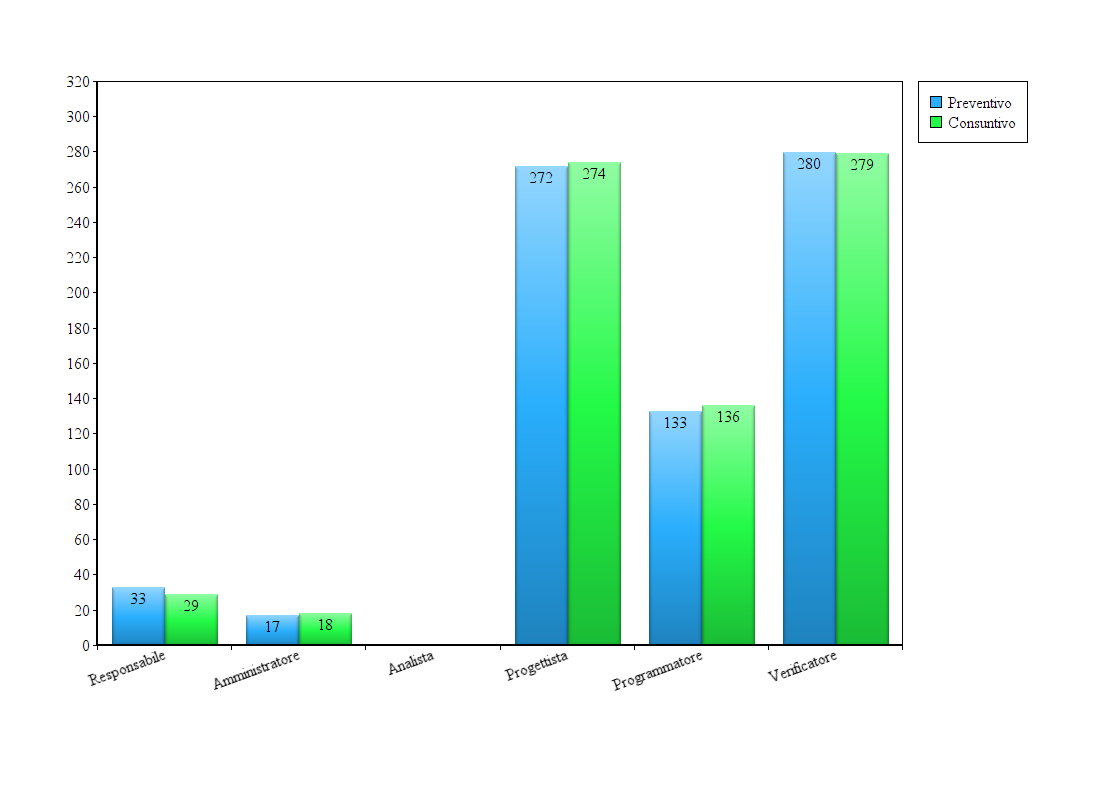
\includegraphics[scale=0.4]{immagini/Grafi/Totale_oreRuolo.png}
	\caption{Differenza preventivo-consuntivo per ruolo, Totale}
\end{figure}
\FloatBarrier

\subsubsection{Conclusioni}
Come si può notare da quanto riportato sopra le ore totali per lo sviluppo del progetto sono conforme a quanto pianificato. Durante lo sviluppo del progetto i ruoli di ogni componente sono stati adattati per necessità, rendendo le ore pianificare uguali alle ore preventivate, ma con costi diversi. \\
Sono state impiegate un totale di 105 ore per ciascun componente, determinando un costo totale di 13468€.